\documentclass[a4paper]{article}

%! Author = syedalimohsinbukhari
%! Date = 9/20/26

% Preamble
\usepackage{geometry}
\usepackage{graphicx}
\usepackage{amssymb}
\usepackage{amsfonts}
\usepackage{booktabs}
\usepackage{amsopn}
\usepackage{amsmath}
\usepackage{amstext}
\usepackage[colorlinks=true,linkcolor=blue,citecolor=blue,urlcolor=blue]{hyperref}
\usepackage[sort&compress, numbers]{natbib}
\usepackage{siunitx}
\usepackage{multirow}

\DeclareSIUnit\solarmass{M_{\odot}}

% Combination-space notation (the 2\varphi_c \pm 2\psi degeneracy) -- every reference to combo A/B
% routes through these four macros so the paper can't drift into mixed notations across files again
% (see experiments/phic_psi_poc-redo/UNDERSTANDING.md \S3.4).
\newcommand{\combo}[1]{\ensuremath{\text{combo}_\text{#1}}}
\newcommand{\comboA}{\combo{A}}
\newcommand{\comboB}{\combo{B}}
\newcommand{\comboAFull}{\ensuremath{\comboA\ (2\varphi_c+2\psi)}}
\newcommand{\comboBFull}{\ensuremath{\comboB\ (2\varphi_c-2\psi)}}

% Circular resultant (mode-collapse diagnostic, defined 002_problem-formulation.tex \S\ref{sec:phicpsi:circular}).
\newcommand{\circr}{\ensuremath{\text{circ}_r}}

% Raw-magnitude health diagnostic: defined as sigma_{head,target} (002_problem-formulation.tex
% \S\ref{sec:phicpsi:circular}) but referred to everywhere it's actually checked against a gate
% (006, 007, 008, 010) by its diagnostic-script/CSV column name, std_ratio -- canonicalized on that
% name so the paper stays greppable against the artifacts it cites.
\newcommand{\stdratio}{\ensuremath{\text{STD}_\text{ratio}}}

% Wrap-aware angular MAE: canonicalized on the diagnostic-script/table column name, ang_MAE, typeset
% like the paper's other code/config identifiers (\texttt{double\_angle}, ...) rather than as
% a hand-built math symbol.
\newcommand{\MAEang}{MAE$_\text{ang}$}

% Loss terms (each currently defined and used once, but macroed for the same reason as everything
% above: one place to fix if the notation ever needs to change).
\newcommand{\Lcirc}{\ensuremath{L_\text{circ}}}
\newcommand{\Lmag}{\ensuremath{L_\text{mag}}}

% Model/trunk identifiers: rendered text is copied verbatim from ../model_labels.py's MODEL_LABELS
% values, the same single source of truth the figures import from -- so a model named in prose or a
% table cell and a model plotted in a figure title always read identically (down to the CNN_baseline/
% CNN_attention subscript). Update both together if either changes.
\newcommand{\pocA}{POC$_\text{A}$}
\newcommand{\pocB}{POC$_\text{B}$}
\newcommand{\Tcn}{TCN}
\newcommand{\cnnAttn}{CNN$_\text{attention}$}
\newcommand{\cnnBaseline}{CNN$_\text{baseline}$}
\newcommand{\inceptionTime}{InceptionTime}
\newcommand{\resnetOneD}{ResNet1D}


\title{On the Recoverability of Coalescence Phase and Polarization Angle from Gravitational-Wave Strain: A Systematically Verified Null Result}
\author{Syed Ali Mohsin Bukhari, Asad Ali}
\date{\today}

\begin{document}
    \maketitle

%    \begin{abstract}
    The coalescence phase $\varphi_c$ and polarization angle $\psi$ of a compact-binary gravitational-wave signal are, for the dominant quadrupole radiation mode, degenerate with each other in the face-on limit: because the injection convention used to generate this population's strain makes $\varphi_c$ enter the waveform doubled, exactly as $\psi$ already does, only a single combination, $2\varphi_c \pm 2\psi$, is constrained there, and the individual angles disentangle only as the system moves toward edge-on.
    We test directly whether a point-estimating deep neural network can recover $\varphi_c$ and $\psi$ from two-detector strain --- individually or through their better-conditioned sum/difference combination --- across five trunk architectures, two head parameterizations, and three magnitude-regularization strengths.
    The answer is a defended null: every configuration converges to the random-guessing baseline on both angles, while the same networks recover chirp mass, merger time, signal-to-noise ratio, and sky position with high fidelity from the same shared representation.
    No model here clears a pre-registered metric-health interpretability gate at any regularization strength tried; the null instead rests on convergence across four independent, ungated checks --- direct inspection of the prediction distributions, a code-level gradient-health trace, a $10{,}000$-permutation label-shuffle bootstrap, and population stratification by inclination and signal-to-noise ratio --- applied uniformly across every down-selected model, and we argue explicitly for why this substitute evidentiary structure is trustworthy rather than assert it.
    Two further findings emerge: one architecture (\cnnAttn) shows a genuine, signal-to-noise-monotonic partial sky-localization skill unrelated to the $\varphi_c/\psi$ question, and the inclination control head --- used throughout as a same-model noise-floor calibration --- is shown to carry a small but statistically real sub-floor signal rather than being clean noise.
    This null does not reopen a settled question: neural posterior estimation already represents this degeneracy correctly by construction, since a full posterior need not commit to a single value for an unidentifiable target.
    What point estimation continues to expose is a practical hazard for point-estimate and hybrid pipelines still built on regression heads of this kind, and a second hazard one level up the diagnostic stack: a passing interpretability gate is not by itself proof that its subject matter is free of the pathology the gate is meant to catch, a lesson this study's own pre-registered retune produced directly, when a checkpoint that cleared every numeric gate threshold turned out, on scatter-plot inspection, to be a literal two-point mode collapse.
\end{abstract}


    \section{Introduction}
    \label{sec:phicpsi:intro}
    Since the first direct detection of gravitational waves from a binary black hole merger~\citep{abbott2016gw150914}, deep-learning approaches to gravitational-wave parameter estimation have matured rapidly, from early proof-of-concept classifiers~\citep{george2018deep} to amortized neural posterior estimators that approach the accuracy of stochastic-sampling pipelines~\citep{gabbard2022vitamin,dax2021dingo} at a fraction of their latency.
Most of this progress has concentrated on parameters that imprint strongly on the observed strain, i.e., the chirp mass~\citep{cutler1994gw}, the merger time and signal-to-noise ratio~\citep{allen2012findchirp}, and the sky position~\citep{fairhurst2009triangulation,singer2016bayestar}.

Two extrinsic parameters have received far less attention as direct regression targets: the orbital phase at coalescence, $\varphi_c$, and the polarization angle, $\psi$.
There is a physical reason for this neglect.
For the dominant quadrupole ($\ell=2$, $|m|=2$) mode of a quasi-circular compact binary, the two polarization states are~\citep{sathyaprakash2009physics}
\begin{equation*}
    \begin{aligned}
    h_+ &\propto (1+\cos^2\iota)\cos\left(2\varphi(t)+2\varphi_c\right),\\
    h_\times &\propto 2\cos\iota\sin\left(2\varphi(t)+2\varphi_c\right),
    \end{aligned}
\end{equation*}
and the detector response mixes them through antenna patterns that depend on $2\psi$~\citep{cutler1994gw,sathyaprakash2009physics}.
Both $\varphi_c$ and $\psi$ enter the strain doubled, so the analytically degenerate combination in the face-on limit ($\cos\iota \to \pm 1$) is $2\varphi_c \pm 2\psi$, with the sign set by the sign of $\cos\iota$.
%The correction traces to how \texttt{coa\_phase} is injected for this population: it is the orbital reference phase in the convention used by the generator, and for a dominant-mode-only waveform that orbital phase enters the strain through $e^{i\cdot 2\cdot\text{coa\_phase}}$, exactly like $\psi$ already does.
In the face-on limit the signal becomes circularly polarized and depends on $\varphi_c$ and $\psi$ only through this single, corrected combination, so the individual angles are exactly unidentifiable there, and only partially disentangled as the inclination moves toward edge-on.
Bayesian samplers absorb this structure into broad, multimodal joint posteriors~\citep{veitch2010bayesian,aasi2013pe,veitch2015lalinference,ashton2019bilby}; a point-estimate regression network has no such refuge.

This paper asks the question:
\begin{quote}
    \itshape Can $\varphi_c$ and $\psi$ be recovered from strain alone by a deep neural network, individually, through their sum/difference combinations, or is the degeneracy effectively exact for a realistic detection-scale population?
\end{quote}

The answer, is a \textbf{null result}: across the five trunk architectures, two head parameterizations, and three values of a magnitude-regularization coefficient.
No model could perform measurably better than random guessing on either angle, while the same networks simultaneously recovered chirp mass, merger time, signal-to-noise ratio, and in some cases, sky position with high fidelity from the same shared features.

A null result of this kind is only as strong as the effort spent trying to break it.
The scientific contribution of this paper is therefore threefold.
First, the null itself, tested against an explicit list of confounds: data-pipeline faults, loss-wiring faults, architecture-specific artifacts, statistical flukes, and population heterogeneity.
Second, a methodological account of \emph{how} the null was established when the standard interpretability gate never cleared --- because unlike a gate failing for one model out of several, here it failed for every model at every regularization strength tried, forcing an explicit argument for why a broader, ungated battery of evidence should be trusted in its place, a response, at engineering-loop scale, to the same replication crisis that motivates pre-registration in quantitative science more broadly~\citep{ioannidis2005false,nosek2018preregistration}.
Third, a methodological lesson demonstrated directly within this study: a checkpoint that cleared every numeric threshold of the pre-registered interpretability gate turned out, on scatter-plot verification, to be a literal two-point mode collapse --- a passing aggregate metric that is not, by itself, proof of the property it is meant to certify.

%This null result carries a direct architectural implication, stated here rather than only in the Discussion.
%Since strain alone does not recover $\varphi_c/\psi$ under point estimation, but \S\ref{sec:phicpsi:prereq}'s analytic study shows the well-constrained combination \emph{is} recoverable given inclination, the natural next step is to condition the network on $\iota$ directly --- scoped as future work in \S\ref{sec:phicpsi:future}.

The research paper is organized as follows;
Section~\ref{sec:phicpsi:problem} formalizes the problem and the circular-regression framework.
Section~\ref{sec:phicpsi:prereq} presents the analytic prerequisite study, rerun under the corrected antenna-pattern model.
Section~\ref{sec:phicpsi:methods} details the datasets, architectures, losses, and training protocol, including the corrected combination construction.
Section~\ref{sec:phicpsi:arc} summarizes, briefly, two optimization pathologies in this training pipeline and how they were fixed prior to the main sweep.
Section~\ref{sec:phicpsi:results} presents the defended null result, its verification battery, and findings.
Section~\ref{sec:phicpsi:prereg} describes the pre-registered magnitude-penalty retune and its outcome.
Section~\ref{sec:phicpsi:discussion} discusses interpretation, limitations, and future work; Section~\ref{sec:phicpsi:conclusion} concludes.



    \section{Problem Formulation}
    \label{sec:phicpsi:problem}
    \subsection{Targets and the degeneracy hypothesis}
\label{sec:phicpsi:targets}

We consider a ten-parameter description of a compact binary coalescence signal injected into two-detector noise: chirp mass $\mathcal{M}$, mass ratio $q$, inclination $\iota$, coalescence phase $\varphi_c$, polarization angle $\psi$, declination, right ascension, injection time, merger time within the analysis window, and network signal-to-noise ratio.
Seven of these are used as supervised regression targets (mass ratio and injection time are excluded; \S\ref{sec:phicpsi:dataset}).
The scientific targets are $\varphi_c \in [0, 2\pi)$, period $2\pi$, and $\psi \in [0, \pi)$, period $\pi$.
Inclination, chirp mass, merger time, SNR, and sky position are retained as \emph{control heads}: parameters trained through the identical pipeline whose success or failure calibrates what the network can extract from strain when information is present.

The degeneracy hypothesis under test is: \emph{$\varphi_c$ and $\psi$ carry no strain-only recoverable signal for this population, in this architecture and loss family}.
A point-estimating network can do no better than the optimal constant prediction.
For most of the population the likelihood constrains only the combination $2\varphi_c \pm 2\psi$, and the remaining direction is unconstrained.
The alternative hypothesis motivating the experimental design is that even if $\varphi_c$ and $\psi$ are individually unrecoverable, their sum and difference combinations may be well-conditioned.
Face-on systems constrain $2\varphi_c \pm 2\psi$ (sign by $\cos\iota$), so a network parameterized in combination space, with a curriculum that weights each combination according to how well the current inclination constrains it, might learn the recoverable structure that a naive per-angle parameterization misses.

%Conditioning on inclination $\iota$ --- tested as future work in \S\ref{sec:phicpsi:future} --- is treated throughout as a \emph{training-paradigm design choice}, motivated by the analytic structure of \S\ref{sec:phicpsi:prereq} showing that the well-constrained combination is recoverable given $\iota$, not as a forced move necessitated by a proof that $\iota$ itself is unrecoverable; \S\ref{sec:phicpsi:inclination} shows $\iota$ in fact carries a small, real signal, which sharpens rather than resolves this question.
%No model in this paper takes $\iota$, or any function of it, as an input at any stage; $\iota$ appears here only as a control \emph{output} head trained on raw strain, exactly like $\varphi_c$ and $\psi$ (\S\ref{sec:phicpsi:circular}).

\subsection{Circular regression framework}
\label{sec:phicpsi:circular}

Periodic targets are regressed on the unit circle~\citep{mardia2000circular}.
An angle $\theta$ with period $T$ is encoded as the two-vector $\mathbf{u}(\theta) = (\sin(2\pi\theta/T), \cos(2\pi\theta/T))$, so the $\psi$ head, with $T=\pi$, physically encodes $2\psi$.
Each periodic head outputs a raw two-vector $\mathbf{v}\in\mathbb{R}^2$, projected onto the unit circle by a normalization layer, $\hat{\mathbf{u}} = \mathbf{v}/\sqrt{\max(\|\mathbf{v}\|^2,\varepsilon)}$, $\varepsilon=10^{-8}$ --- a clamp on the squared norm, for a stable gradient at $\mathbf{v}=\mathbf{0}$, rather than a floor on $\|\mathbf{v}\|$ itself --- and trained with the cosine (circular) loss $\Lcirc = 1 - \hat{\mathbf{u}}_{\text{pred}}\cdot\mathbf{u}_{\text{true}} = 1-\cos\Delta\theta$.

For uniformly distributed targets and any fixed prediction, the expected circular loss is exactly 1; the expected wrap-aware angular mean absolute error (\MAEang) is $T/4$, i.e., $\pi/2 \approx 1.5708$~rad for $\varphi_c$ and $\iota$, $\pi/4 \approx 0.7854$~rad for $\psi$.
These values are the null baselines against which every result in this paper is judged.

Two further diagnostic statistics recur throughout: the circular resultant $\circr = \|\text{mean}(\hat{\mathbf{u}})\|$, which measures mode collapse ($\circr \to 1$ means all predictions concentrate at one angle), and $\sigma_\text{head, target}$, the ratio of the standard deviation of a head's raw outputs to that of the encoded targets, a monitor of raw-magnitude health with a healthy band of $[0.5, 2.0]$ --- called \stdratio\ in the diagnostic chapters from \S\ref{sec:phicpsi:prereg} onward.
Non-periodic heads use a Huber loss on transformed targets, and the sky-position head uses a closed-form von~Mises--Fisher negative log-likelihood on the unit sphere~\citep{fisher1953dispersion}.
One head cuts across this taxonomy: the inclination head keeps the periodic two-vector encoding but its loss is Huber on the raw output vector, with no normalization and no circular loss anywhere in its path.
All heads share a single trunk and are combined by learned homoscedastic uncertainty weighting~\citep{kendall2018multi}.



    \section{Prerequisite Study}
    \label{sec:phicpsi:prereq}
    Before any training, the combination-space hypothesis was tested analytically, using a toy detector-response model in which $h_+$/$h_\times$ add $2\varphi_c$ to the orbital-phase term $2\Phi$.
A required self-check --- sweeping $\psi$ at fixed $2\varphi_c+2\psi$, confirming $(R,\delta)$ stays exactly constant at $\iota=0$ --- passed to machine precision ($\max\,\text{std}(R)=1.16\times10^{-14}$, $\max\,\text{std}(\delta)=5.87\times10^{-16}$), gating trust in everything that follows.

The 100-point inclination sweep (50 points per sign of $\cos\iota$, 200 sky positions, 5{,}000-draw bootstrap) confirms the expected combination structure:
\begin{itemize}
    \item for $\cos\iota>0$, \comboBFull\ is the better-constrained combination throughout; for $\cos\iota<0$, \comboAFull\ wins --- a clean sign flip driven by the sign of $\cos\iota$;
    \item the preference ratio is strongest face-on, $\approx1.62$--$1.65\times$, decaying monotonically to $\approx1.04$--$1.07\times$ at edge-on, never crossing 1.0;
    \item population-bootstrapped mean ratios are $1.17\times$ (95\% CI $[1.11,1.24]$) for $\cos\iota>0$ and $1.19\times$ (95\% CI $[1.12,1.26]$) for $\cos\iota<0$, with the simple two-point reference check clearing significance directly.
\end{itemize}

The sign flip described above and the monotonic decay in the preference ratio share one mechanical cause.
The toy model's two antenna-weighted amplitude coefficients respond asymmetrically to inclination: $k_1(\iota)=(1+\cos^2\iota)/2$ for $h_+$ stays strictly positive across $[0,\pi]$, while $k_2(\iota)=\cos\iota$ for $h_\times$ crosses zero at $\iota=\pi/2$ and changes sign on either side.
Since the detector strain is $F_+h_++F_\times h_\times$, that sign change in $h_\times$'s own amplitude is what flips which of \comboA/\comboB\ the strain constrains more tightly, and the same vanishing of $k_2$ at edge-on is why the preference ratio closes toward $1.0\times$ there: with $h_\times$'s contribution suppressed, the two combinations become comparably constrained rather than either one standing out.
The ratio peaks at face-on instead, where $k_1$ and $k_2$ are both near their maximum magnitude and the signal is closest to circularly polarized.

Which combination wins for a given sign of $\cos\iota$ is read off empirically from the correlation sweep itself, not assumed in advance from the coefficient asymmetry alone.
That distinction is not academic: this redo's \comboA/\comboB\ use the corrected construction of \S\ref{sec:phicpsi:heads} (angle $2\varphi_c\pm2\psi$, via an explicit doubling of the $\varphi_c$ head before combination), and an earlier, uncorrected version of this experiment found \comboB\ well-constrained for a differently-defined pair (\texttt{formulae\_reference.md} \S A.2) --- a finding this redo deliberately did not carry forward, re-deriving the sign assignment empirically under the corrected formula instead.

\begin{figure}[tbp]
    \centering
    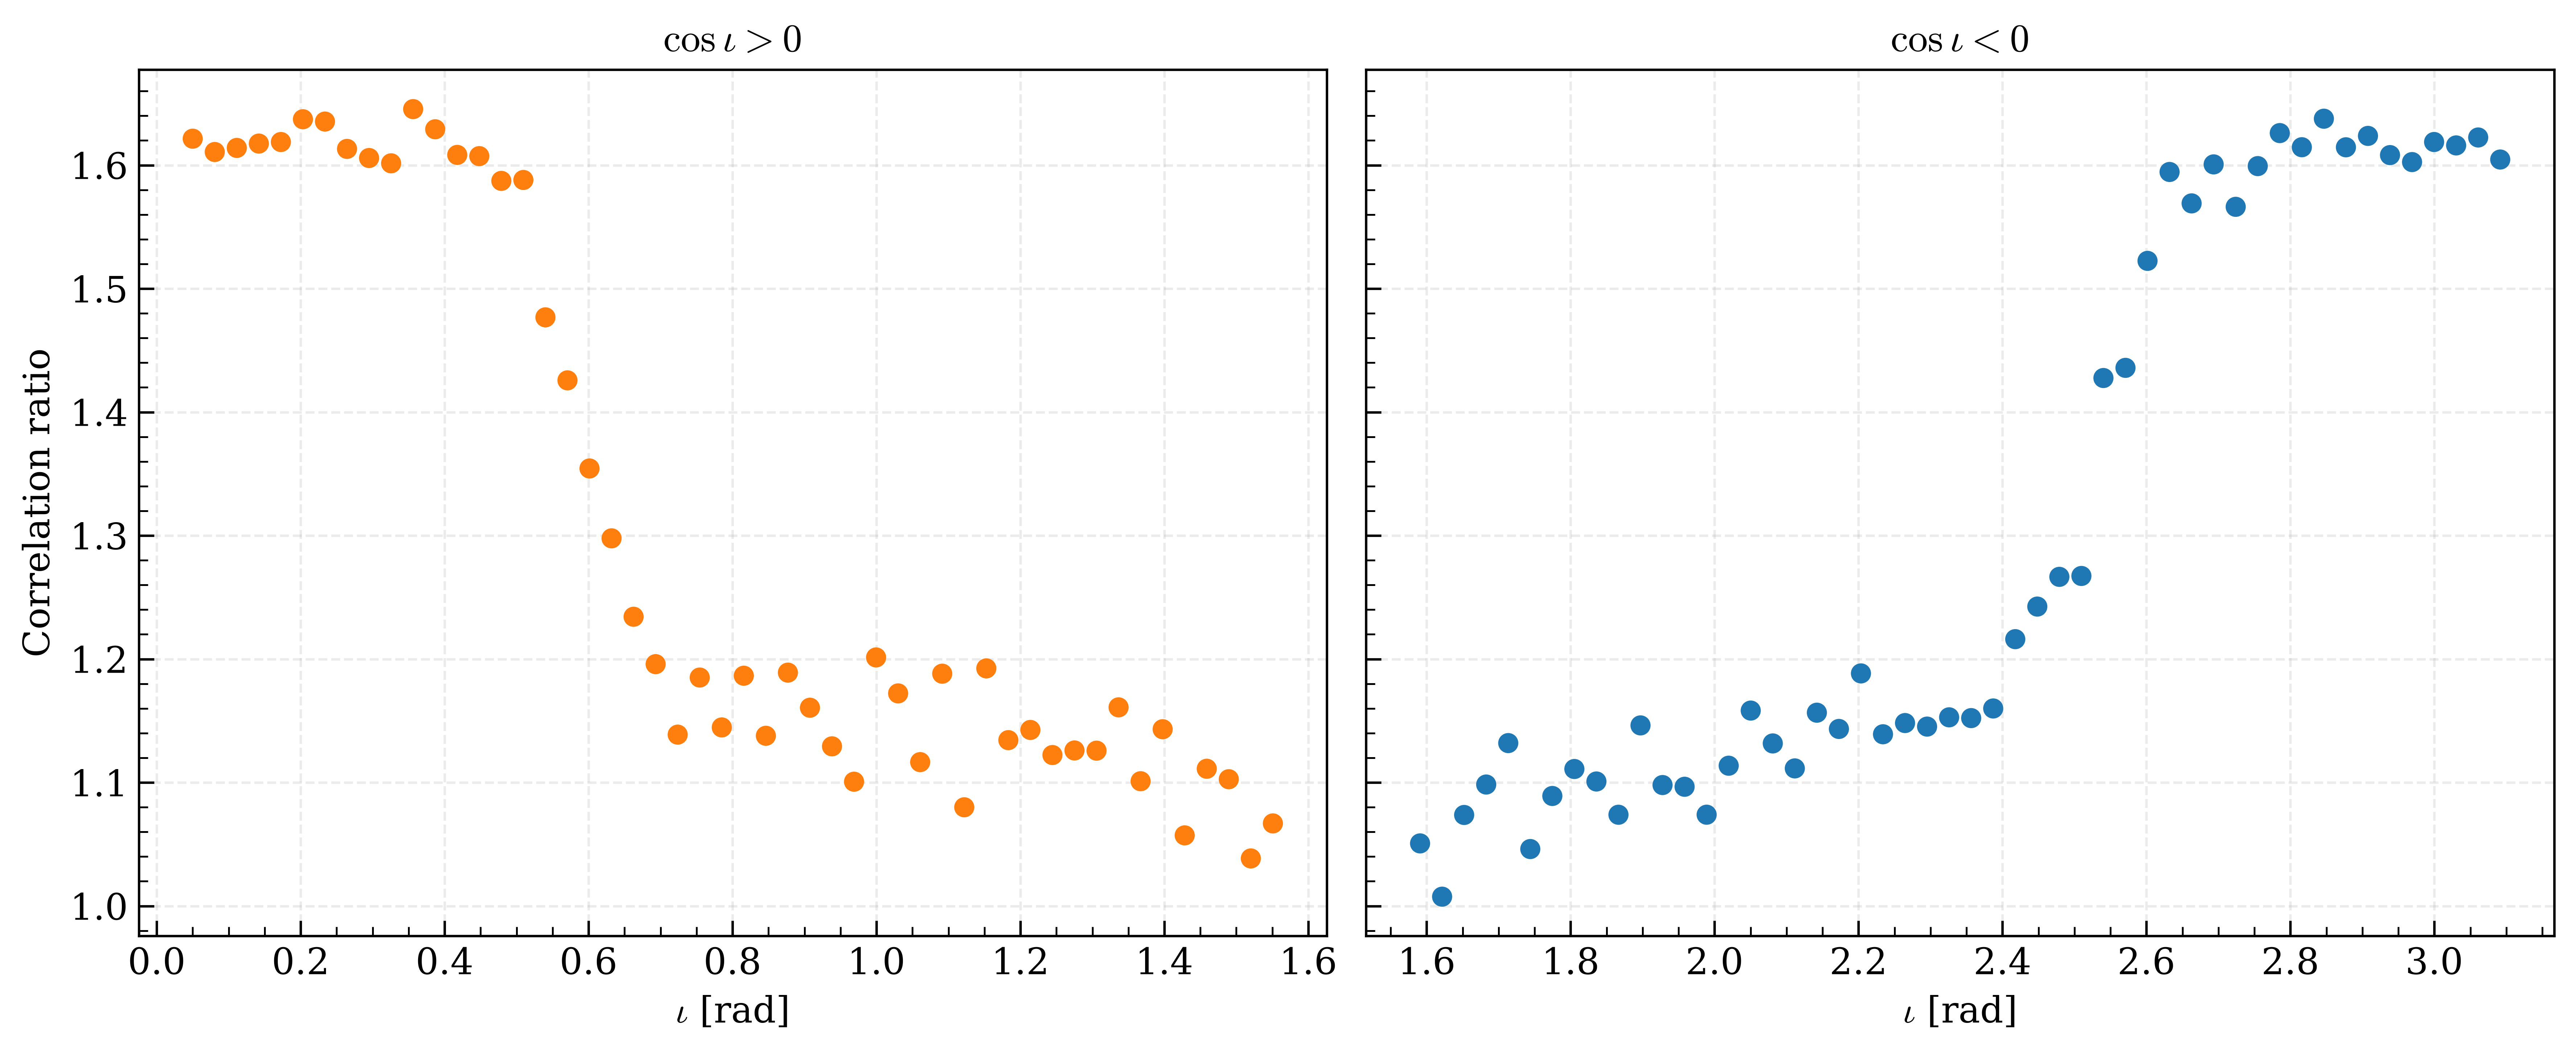
\includegraphics[width=\columnwidth]{sweep_1_1_ratio_vs_iota.png}
    \caption[Analytic check of the corrected degeneracy structure]{Analytic check of the corrected $2\varphi_c$--$2\psi$ degeneracy structure: ratio of the strain correlation with the well-constrained combination to the poorly-constrained one, as a function of inclination.}
    \label{fig:sweep}
\end{figure}

The curriculum weight derivation gives $w(\text{face-on})=0.0000$ and $w(\text{edge-on})=0.1416$, with an intermediate-peak shape; training uses the analytically motivated fallback $w(\iota)=1-\cos^2\iota=\sin^2\iota$ rather than the fitted empirical curve.
Population balance: 28.7\% of samples are near-face-on ($|\cos\iota|>0.9$), 32.7\% near-edge-on ($|\cos\iota|<0.5$).



    \section{Methods}
    \label{sec:phicpsi:methods}
    \subsection{Dataset}
\label{sec:phicpsi:dataset}

All experiments use a single pre-generated HDF5 dataset of simulated two-detector observations: \num{25000} training and \num{5000} validation samples, each a pair of \num{4096} sample noisy strain series for the H1 and L1 detectors --- a 2\,s window at \SI{2048}{\hertz} --- stacked as a $(4096,2)$ input tensor.
All injections use the dominant quadrupole ($\ell=2$, $|m|=2$) mode only (IMRPhenomD), with no higher-order modes.
%This detail, and the injection convention behind the combination formula of \S\ref{sec:phicpsi:intro}, is traced directly through the dataset's generator source code rather than recorded from recollection; the dataset itself was not regenerated from a version-controlled generator, so a reproducibility gap remains open (\S\ref{sec:phicpsi:future}).
Table~\ref{tab:population} gives the marginal parameter distributions.

\newcommand{\mrows}[2]{\multirow{#1}{*}{#2}}

\begin{table}[tbp]
    \centering
    \caption{Marginal parameter distributions for the injected population.}
    \label{tab:population}
    \small
    \begin{tabular}{@{}ccl@{}}
        \toprule
        Parameter & Support & Distribution \\
        \midrule
        $m_1$ & $10$--$50\,M_\odot$ & Uniform pair\\
        $m_2$ & $10$--$50\,M_\odot$ & Uniform pair\\
        $q=m_2/m_1$ & \mrows{2}{$0.20$--$1.00$} & \mrows{2}{Derived} \\
        $m_1\geq m_2$ & & \\
        $\mathcal{M}$ & $8.84$--$43.45\,M_\odot$ & Derived \\
        SNR & $[7,15]$ & Uniform \\
        $\varphi_c$ & $[0,2\pi)$ & Uniform \\
        $\psi$ & $[0,\pi)$ & Uniform \\
        $\iota$ & $[0,2\pi)$ & Uniform in $\iota$ \\
        Right ascension & $[0,2\pi)$ & Uniform \\
        Declination & $[-\pi/2,\pi/2]$ & $\cos$ weighted \\
        \bottomrule
    \end{tabular}
\end{table}

Component masses are drawn via two independent $\mathrm{Uniform}(10,50)\,M_\odot$ values, sorted so $m_1\geq m_2$.
These drawn values were than used to derive both mass ratio and chirp mass.

The important parameter here is the inclination angle ($\iota$).
The parameter distribution is uniform in itself, over-representing face-on systems and under-representing edge-on systems relative to a truly isotropic population.
Because face-on is where the $\varphi_c/\psi$ degeneracy is strongest, this skew could in principle bias a \emph{pooled} statistic --- one averaged across the whole population, such as \S\ref{sec:phicpsi:results}'s headline circular-loss numbers --- mildly toward looking like a null, simply by weighting more hard-to-recover cases into the average.
That possibility cannot explain the null result itself: the inclination-band stratification of \S\ref{sec:phicpsi:inclination} measures recovery within each band separately, so the population mix has no opportunity to act on it, and even the edge-on band, checked in isolation, clears no recovery above the materiality floor either.
The strain is than fed to the model already whitened; targets are transformed per \S\ref{sec:phicpsi:circular} on training-split statistics.

\subsection{Trunk architectures}
\label{sec:phicpsi:trunks}

\begin{sloppypar}
Five one-dimensional trunk architectures were evaluated, all mapping the $(4096,2)$ input to a pooled feature vector shared by every head: a temporal convolutional network (\Tcn, primary, dilated residual blocks, receptive field $\approx$ full window~\citep{bai2018tcn}), a plain hierarchical CNN (\cnnBaseline), a strided-conv-plus-transformer network with learned attention pooling (\cnnAttn~\citep{vaswani2017attention}), a multi-scale-kernel network (\inceptionTime~\citep{fawaz2019inceptiontime}), and a residual network (\resnetOneD~\citep{he2016resnet}).
\end{sloppypar}
These five were chosen as five distinct inductive-bias families, not five samples from one family, so that each represents a different hypothesis about how phase information might be encoded in the strain.
Each head is a two-layer MLP (64 hidden units, ReLU) on the shared features, with a linear 2-unit output for periodic heads.

\subsection{Head parameterizations under the corrected formula}
\label{sec:phicpsi:heads}

\textbf{Baseline mode} uses independent circular-loss heads directly on $\varphi_c$ and $\psi$, each with its own uncertainty weight; the named configuration \pocA is baseline mode on the \Tcn trunk.
\textbf{PoC mode} (named configuration \pocB, also on \Tcn) constructs the two combination heads explicitly rather than treating $\varphi_c$ and $\psi$ as independent outputs.
The $\varphi_c$ head's unit vector, $\mathbf{z}_{\varphi_c}$, is first passed through a \texttt{double\_angle} operation, $\mathbf{z}_{2\varphi_c} = \mathbf{z}_{\varphi_c} \otimes \mathbf{z}_{\varphi_c}$ (complex multiplication of the vector with itself), which turns a unit vector at angle $\varphi_c$ into one at angle $2\varphi_c$; the $\psi$ head's own encoding already stores $2\psi$ internally (\S\ref{sec:phicpsi:circular}).
The two combination vectors are $\mathbf{z}_A = \mathbf{z}_{2\varphi_c}\otimes\mathbf{z}_\psi$ (angle $2\varphi_c+2\psi$) and $\mathbf{z}_B = \mathbf{z}_{2\varphi_c}\otimes\overline{\mathbf{z}_\psi}$ (angle $2\varphi_c-2\psi$).
The isotropic circular loss, sign-dependent per-sample curriculum weighting, and uncertainty-weighting scheme are fixed pipeline components, applied identically to every head.
The well-constrained combination assignment (\comboB\ for $\cos\iota\geq0$) is derived from this study's own prerequisite analysis (\S\ref{sec:phicpsi:prereq}).

\subsection{Magnitude penalty}
\label{sec:phicpsi:penalty}

Following the diagnosis in \S\ref{sec:phicpsi:arc}, all configurations add an explicit radial regularizer on the raw, pre-normalization periodic outputs, $\Lmag = \lambda \cdot \sum \text{mean}[(\|\mathbf{v}\|-1)^2]$, present in every configuration from the first training run.
$\lambda=0.01$ for the main sweep (\S\ref{sec:phicpsi:results}), retuned to 0.05 and 0.10 in \S\ref{sec:phicpsi:prereg}.

\subsection{Training protocol}
\label{sec:phicpsi:protocol}

Adam, initial learning rate $10^{-3}$, \texttt{ReduceLROnPlateau} (factor 0.5, patience 5), batch size 128, 80 epochs, seed 42, uncertainty weighting with log-variance clamp $\pm3$, Huber $\delta=1$.
Periodic epoch-10 checkpoints were saved throughout, not only best/final weights.

\subsection{Evaluation}
\label{sec:phicpsi:evaluation}

Point predictions are scored by wrap-aware angular MAE, $\circr$, and, for scalar heads, MAE/$R^2$.
Statistical significance is assessed by a label-permutation bootstrap ($N=10{,}000$ shuffles), and population heterogeneity is probed by SNR-tercile and inclination-band stratification.
Two additional checks were added in response to a genuine new finding for one architecture (\S\ref{sec:phicpsi:sky}) rather than planned in advance: a formal shuffle-null bootstrap and SNR-tercile stratification for the sky-position head's own angular separation.



    \section{Inherited Diagnostic History and Present-Day Machinery Check}
    \label{sec:phicpsi:arc}
    \subsection{Two optimization pathologies and their fixes}
\label{sec:phicpsi:inherited}

Before any measurement of the degeneracy could be trusted, two genuine optimization pathologies in this training pipeline had to be found and fixed: tanh saturation at random initialization on the periodic head output layers, fixed by switching to a linear output activation since the unit-circle normalization already handles projection; and, once that was fixed, a second pathology in which the isotropic circular loss provides no restoring force on the raw output's magnitude, so the normalization layer's backward pass either crushes or explodes the angular gradient as the magnitude drifts, fixed by the explicit magnitude penalty of \S\ref{sec:phicpsi:penalty}.
Both are established facts about this codebase's training mechanism, fixed before the main sweep in \S\ref{sec:phicpsi:results} began; that sweep does not re-narrate the bug hunt that found them.

\subsection{Verification on trained checkpoints}
\label{sec:phicpsi:verification}

Confirming, on the Round-1 ($\lambda=0.01$) checkpoints, that the machinery above is healthy is a prerequisite to trusting anything it produces.
True labels are clean (circular resultant $\leq 0.013$ for $\varphi_c/\psi/\iota$/right ascension).
Gradients reach the periodic-head weights end to end through the corrected construction: $dL/d($\comboA$) = 0.4245$, dropping through the \texttt{double\_angle} stage ($dL/d(\mathbf{z}_{2\varphi_c,\text{norm}})=0.375$) to $dL/d(\mathbf{z}_{\varphi_c,\text{raw}})=0.570$ and $dL/d(\mathbf{z}_{\psi,\text{raw}})=0.514$ --- comparable in order of magnitude to the healthy inclination-head baseline, 0.728.
Positive controls recover well (Fig.~\ref{fig:controls}): chirp mass $R^2=0.920$--$0.960$, merger time $R^2=0.906$--$0.928$, SNR $R^2=0.741$--$0.789$, sky position $4.4^\circ$--$10.3^\circ$ mean angular error.

\begin{figure}[tbp]
    \centering
    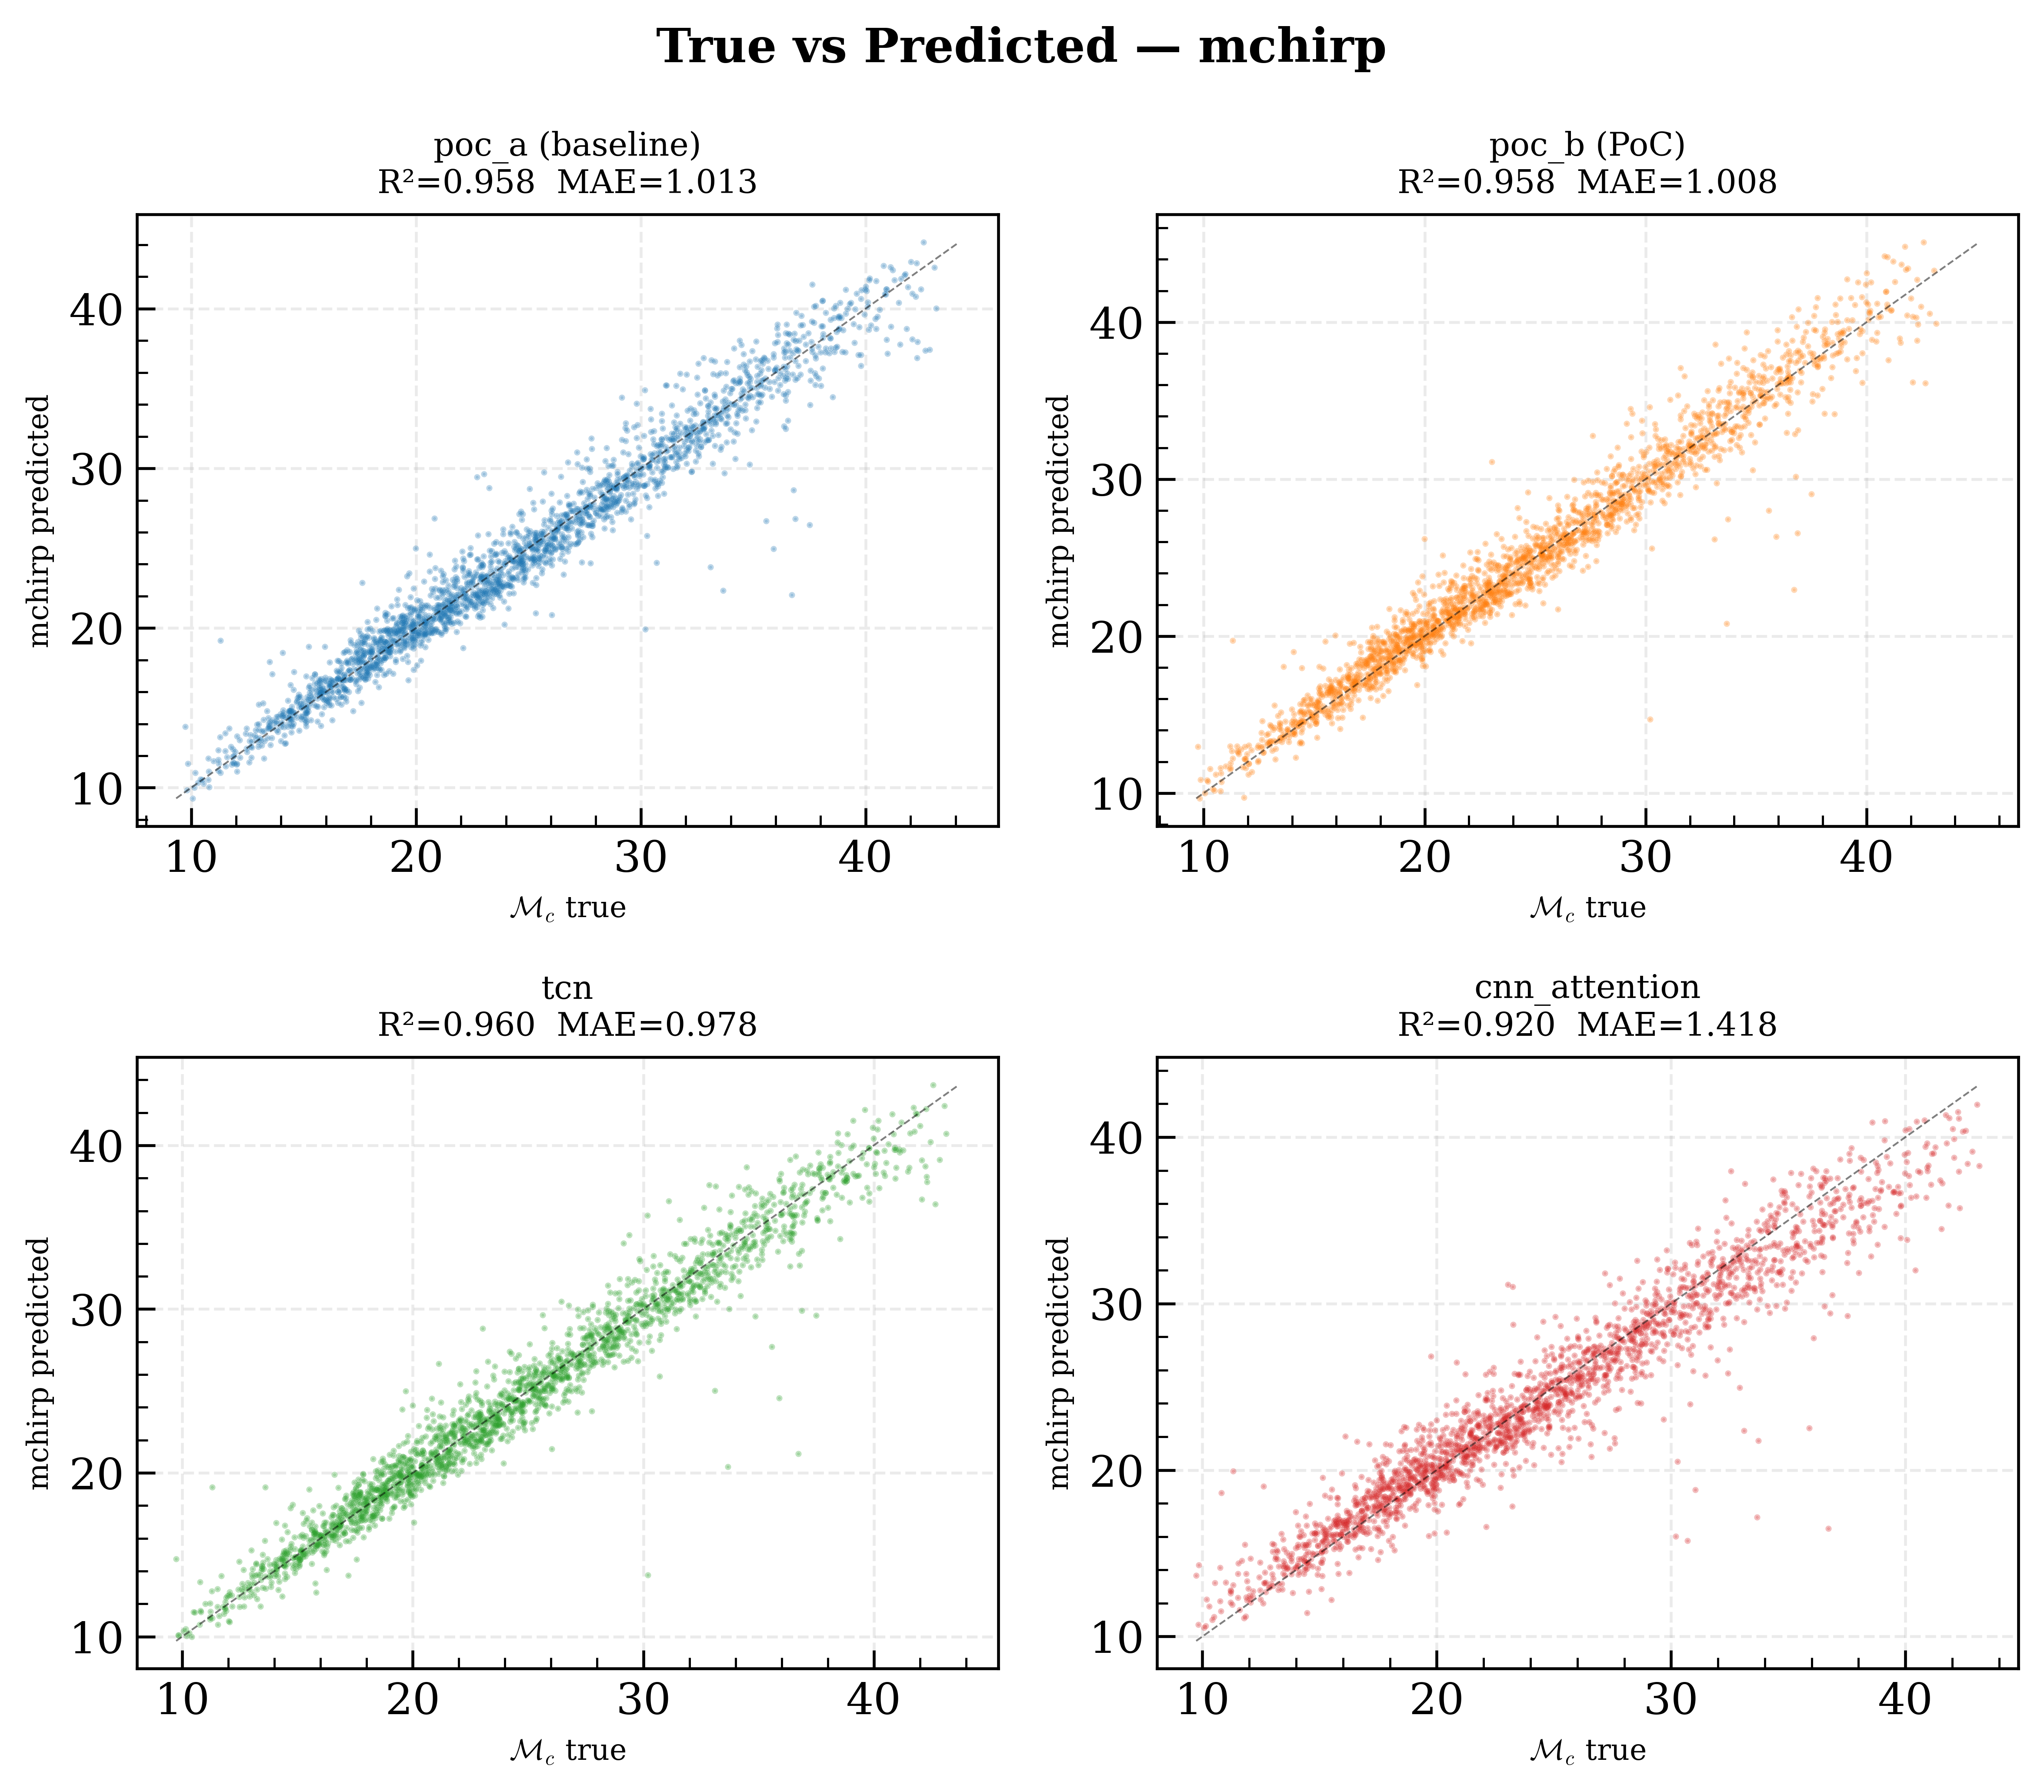
\includegraphics[width=\columnwidth]{scatter_mchirp_20260916_113847.png}
    \caption{Positive-control recovery (chirp mass) for the four down-selected models.}
    \label{fig:controls}
\end{figure}

The machinery this study depends on is verifiably healthy; what it produces on the question of interest is presented next.



    \section{Results: A Defended Null, Under the Corrected Formula}
    \label{sec:phicpsi:results}
    \subsection{Headline result}
\label{sec:phicpsi:headline}

At epoch 79 (last-10-epoch mean), \pocB's combination-space circular loss reads $\comboA=0.9999$, $\comboB=0.9895$ --- both essentially at the ceiling value of 1 expected under random guessing.
Table~\ref{tab:headline} reports angular recovery for all four down-selected models at $\lambda=0.01$.

\begin{table}[tbp]
    \centering
    \caption{Periodic-head recovery, four down-selected models, $\lambda=0.01$.}
    \label{tab:headline}
    \small
    \begin{tabular}{@{}llccc@{}}
        \toprule
        Head & Model & $\circr$ & \MAEang & Grade \\
        \midrule
        $\varphi_c$ & \pocA & 0.542 & 1.586 & XX \\
        $\varphi_c$ & \pocB & 0.975 & 1.535 & \textbf{COLLAPSE} \\
        $\varphi_c$ & \Tcn & 0.840 & 1.590 & XX \\
        $\varphi_c$ & \cnnAttn & 0.386 & 1.616 & XX \\
        $\psi$ & \pocA & 0.972 & 0.801 & \textbf{COLLAPSE} \\
        $\psi$ & \pocB & 1.000 & 0.801 & \textbf{COLLAPSE} \\
        $\psi$ & \Tcn & 0.639 & 0.799 & $\sim$ \\
        $\psi$ & \cnnAttn & 0.396 & 0.785 & $\sim$ \\
        \bottomrule
    \end{tabular}
\end{table}

\pocA and \pocB are, by a systematic COLLAPSE grade ($\circr>0.9$ \emph{and} \MAEang$>0.5$), genuinely mode-collapsed: \pocB's $\psi$ predictions place 99.9\% of 5{,}000 validation samples in one $10^\circ$-wide histogram bin.
\Tcn and \cnnAttn fail differently --- noisy and uninformative rather than collapsed --- but \MAEang\ sits at the null for both.
A direct forward-pass check makes the collapse concrete: three \comboA predictions from very different true angles ($-1.45,-2.22,+1.76$~rad) come back at $1.468,1.496,1.499$~rad regardless of input.

\subsection{Confound elimination}
\label{sec:phicpsi:confounds}

Loss wiring is confirmed correct in both training modes by direct code trace, not by inspecting a misleadingly generic loss-dictionary listing.
The gradient path is confirmed live end to end (\S\ref{sec:phicpsi:verification}).
The collapse is confirmed genuine, not a metric artifact, by direct histogram inspection (\S\ref{sec:phicpsi:headline}).
This study's own pre-registered interpretability gate (\S\ref{sec:phicpsi:prereg}) never clears at any $\lambda$ tried, so these confound checks are reported directly against the trained checkpoints rather than inferred from a passing gate --- an evidentiary substitution argued explicitly in \S\ref{sec:phicpsi:reconcile}.

\subsection{Statistical significance}
\label{sec:phicpsi:bootstrap}

\begin{table}[tbp]
    \centering
    \caption{Label-permutation bootstrap ($N=10{,}000$, one-sided). $z>0$: better than shuffled-null.}
    \label{tab:bootstrap}
    \small
    \begin{tabular}{@{}lccc@{}}
        \toprule
        Model & $\varphi_c$: $z,p$ & $\psi$: $z,p$ & $\iota$: $z,p$ \\
        \midrule
        \pocA & $-0.38$, .649 & $-0.82$, .793 & $+2.00$, .0223 \\
        \pocB & $-0.39$, .649 & $-0.63$, .740 & $+2.58$, .0052 \\
        \Tcn & $-1.18$, .879 & $-0.50$, .692 & $+2.58$, .0059 \\
        \cnnAttn & $-1.97$, .976 & $+1.33$, .091 & $+3.58$, .0003 \\
        \bottomrule
    \end{tabular}
\end{table}

$\varphi_c$ and $\psi$: 0 of 8 tests significant, most worse than chance.
$\iota$ reads significant in all four models at the uncorrected $\alpha=0.05$ level, but applying a 12-test Bonferroni correction ($0.05/12\approx0.00417$) leaves only \cnnAttn's $p=0.0003$ surviving; \pocA ($p=0.0223$), \pocB ($p=0.0052$), and \Tcn ($p=0.0059$) do not.
Inclination therefore carries a statistically real signal in one model under correction, and a signal significant only uncorrected in the other three --- in every case with an effect size (\S\ref{sec:phicpsi:inclination}) well below this study's own materiality floor of 0.10~rad.

\subsection{SNR stratification}
\label{sec:phicpsi:snr}

No head/model combination clears the 0.10~rad floor in the high-SNR tercile for $\varphi_c$ or $\psi$.
\Tcn/$\varphi_c$ is the sole monotonic-with-SNR improver ($\Delta=+0.0209$~rad at high SNR), but it is the one model whose \stdratio\ never stabilizes at any $\lambda$ (\S\ref{sec:phicpsi:prereg}), so its trend is dismissed as doubly uninterpretable, not merely small.

\subsection{Loss trajectory and failure signature}

Across all 80 epochs, combination-space circular loss is flat within noise for every model.
The failure signature these checkpoints show is \stdratio\ settling low from early training (\S\ref{sec:phicpsi:prereg}), not validation loss creeping upward late.

\subsection{The perturbation-trace probe: parked, not closed}

This study's calibration stage for the multi-step perturbation trace failed on its own pre-declared terms for every one of the four models: the mchirp positive control never reads directional even under favorable fresh-init conditions, so the probe's verdicts on the heads under test cannot be trusted.
No salvage was attempted; the probe is stated as parked, not closed, and carried forward as future work (\S\ref{sec:phicpsi:future}).

\subsection{Inclination: a small, real, sub-floor signal --- not a clean noise floor}
\label{sec:phicpsi:inclination}

Inclination was used throughout as a same-model noise-floor calibration for judging $\varphi_c/\psi$'s own band-to-band deviations, on the premise that its apparent failure was clean noise.
That premise does not survive this study's bootstrap evidence: $\iota$ carries a small, real signal (\S\ref{sec:phicpsi:bootstrap}), with an effect size of roughly 0.02--0.04~rad, verified against the underlying scatter plots and not the $p$-value alone.
No $\varphi_c/\psi$ deviation, face-on to edge-on, clears the 0.10~rad floor in either direction for any model; a companion check on a non-angular control (chirp mass, banded identically) shows small band-to-band spread, ruling out the banding scheme itself as an alternative explanation.

\subsection{A new finding: \cnnAttn's partial sky-localization skill}
\label{sec:phicpsi:sky}

Sky position was carried throughout as a positive control; here it is tested for significance directly.

\begin{table}[tbp]
    \centering
    \caption{Sky-position angular separation.}
    \label{tab:sky}
    \small
    \begin{tabular}{@{}lccl@{}}
        \toprule
        Model & Bootstrap $\Delta$ (deg), $z$ & High-SNR $\Delta$ & Verdict \\
        \midrule
        \pocA & 3.43, $+6.54\sigma$ & $+3.01$ & sub-floor \\
        \pocB & 3.03, $+5.51\sigma$ & $+2.90$ & sub-floor \\
        \Tcn & 2.86, $+5.21\sigma$ & $+2.53$ & sub-floor \\
        \cnnAttn & \textbf{12.58}, $\mathbf{+23.23\sigma}$ & \textbf{+15.53} & \textbf{real-recovery} \\
        \bottomrule
    \end{tabular}
\end{table}

Three models show the same small-but-real, sub-floor pattern as inclination.
\begin{sloppypar}
\cnnAttn clears the materiality floor outright, and --- since this model is independently known to memorize $\varphi_c/\psi$ training-set structure without generalizing (\S\ref{sec:phicpsi:pool}) --- the SNR discriminator resolves in favor of genuine recovery, not memorization: a hypothetical population-mean predictor scores only $\approx89.4^\circ$ (essentially at the null), and the actual error shrinks monotonically with SNR ($80.15^\circ\to77.95^\circ\to74.47^\circ$).
\end{sloppypar}
The leading mechanism hypothesis is cross-detector H1/L1 amplitude-ratio information via the sky-dependent antenna pattern --- an envelope cue, not carrier phase --- so this finding is peripheral to, and does not affect, the $\varphi_c/\psi$ null.



    \section{The Pre-Registered $\lambda$ Retune}
    \label{sec:phicpsi:prereg}
    \subsection{Why pre-register}

This study adopted a strict pre-registration discipline from the outset, after a small cautionary episode of its own: on one same-day instance, an uncertainty-weight trajectory was misread by eye and had to be corrected with a mechanical check before any retune began.
The criterion was written down --- a Step~0 \stdratio\ gate, a Bonferroni-corrected bootstrap on the combination angles, a 0.10~rad effect-size floor, and an SNR-monotonicity check --- before any $\lambda=0.05/0.10$ result existed.
Because the combination construction depends on both source vectors jointly, the gate requires all four readings (both heads, poc-mode and baseline-mode) to pass; a single failing reading keeps the whole round uninterpretable.

\subsection{Outcome across three $\lambda$ values}

\begin{table}[tbp]
    \centering
    \caption{Step~0 gate, all three $\lambda$ rounds, all four readings.}
    \label{tab:gate}
    \small
    \begin{tabular}{@{}llcc@{}}
        \toprule
        $\lambda$ & Reading & final $\stdratio$ & Gate \\
        \midrule
        0.01 & \pocB / $\varphi_c$ & 0.583 & FAIL \\
        0.01 & \pocB / $\psi$ & 0.251 & FAIL \\
        0.01 & \pocA / $\varphi_c$ & 0.407 & FAIL \\
        0.01 & \pocA / $\psi$ & 0.374 & FAIL \\
        0.05 & \pocB / $\varphi_c$ & 0.315 & FAIL \\
        0.05 & \pocB / $\psi$ & 0.531 & FAIL \\
        0.05 & \pocA / $\varphi_c$ & 0.522 & FAIL \\
        0.05 & \pocA / $\psi$ & 0.572 & FAIL \\
        0.10 & \pocB / $\varphi_c$ & 0.930 & PASS* \\
        0.10 & \pocB / $\psi$ & 0.421 & FAIL \\
        0.10 & \pocA / $\varphi_c$ & 0.546 & FAIL \\
        0.10 & \pocA / $\psi$ & 0.559 & FAIL \\
        \bottomrule
    \end{tabular}
\end{table}

*The one nominal PASS does not survive inspection.
\pocB's $\varphi_c$ at $\lambda=0.10$ clears every numeric gate threshold, but its own training-time scatter plot shows two completely flat horizontal bands at the same angle modulo $2\pi$ --- a literal two-point mode collapse present from epoch~5 through epoch~80, not real per-sample learning.
\stdratio\ certifies raw-vector norm health, not angular diversity, and the two are not interchangeable: nothing about clearing the numeric threshold guarantees the scatter plot will look healthy.

With every reading at $\lambda=0.10$ either failing outright or failing on inspection, the round closes: $\lambda$ alone is insufficient to stabilize this pipeline's $\|v\|$-space for these heads.
Steps beyond the gate never ran, because the gate never cleared at any $\lambda$, for any of the twelve readings.
Per the pre-registered decision table, this is filed as \textbf{uninterpretable}, not as a null result and not as counter-evidence, on its own narrow terms --- a negative result about the retune mechanism, not the basis for this paper's headline conclusion (\S\ref{sec:phicpsi:results}); \S\ref{sec:phicpsi:reconcile} reconciles the two.



    \section{Discussion}
    \label{sec:phicpsi:discussion}
    \subsection{Reconciling two lines of evidence that do not collapse into one}
\label{sec:phicpsi:reconcile}

This study's own two lines of evidence do not collapse into one, and the tension between them is argued here rather than asserted away.
A pre-registered metric-health gate (\S\ref{sec:phicpsi:prereg}) was meant to license a clean, certified test of the degeneracy: no model, at any $\lambda$, ever passed it --- there is no certified subset of any size to build that argument on.

The null in \S\ref{sec:phicpsi:results} instead rests on four independent methods --- collapse/histogram inspection, a gradient-health trace, a formal bootstrap, and population stratification --- run uniformly across all four down-selected models, without excluding any on interpretability grounds.
This substitution answers a different, and in some ways more direct, question than the gate does: not whether a specific combination vector's raw magnitude is well behaved, but whether these checkpoints' actual predictions carry recoverable signal --- and the collapse and gradient-chain evidence rule out an implementation bug as the cause by a more direct method than gate-passage ever provided.
It is also, we state plainly, a novel evidentiary structure that has not previously been scrutinized in this form.
A skeptical reader is entitled to ask whether an ungated battery, assembled after the pre-registered path proved terminal, is a second attempt dressed as independent confirmation.
It is a different, not a repeated, attempt: several of its components (the gradient-chain trace, the raw histogram inspection) are not calibrated against any threshold chosen after seeing data and simply report what is there --- but the reactive order of construction is a real, stated limitation on how much independent confirmatory weight it should carry relative to a fully pre-registered test.

\subsection{Sufficiency of the architecture pool}
\label{sec:phicpsi:pool}

The five trunk families were chosen as five distinct inductive-bias hypotheses, not five samples from one family, and capacity is not the binding constraint: the memorization-gap check, run uniformly across all four down-selected models, shows \cnnAttn's training-split circular loss falling to 0.54--0.56 by epoch~80 while validation stays flat at $\approx1.0$ (train--val gap $+0.44$ to $+0.47$), against gaps an order of magnitude smaller for the other three models ($+0.003$ to $+0.05$).
\cnnAttn demonstrably has, and uses, spare capacity to fit sample-specific noise on $\varphi_c/\psi$ and generalizes none of it --- while simultaneously showing genuine, generalizing skill on sky position (\S\ref{sec:phicpsi:sky}), illustrating that this model's capacity is head-specific, not uniformly wasted or informative.

\subsection{Relation to full-posterior methods}
\label{sec:phicpsi:npe}

This null does not reopen a settled question.
Neural posterior estimation --- conditional variational autoencoders~\citep{gabbard2022vitamin}, direct neural posterior-density approximations~\citep{chua2020learning,green2020complete}, and conditional normalizing flows trained by simulation-based inference~\citep{papamakarios2021normalizing,cranmer2020frontier,dax2021dingo,dax2023dingois} --- does not attempt a single value for a parameter the likelihood only partially constrains; it learns an amortized approximation to the full posterior and reproduces multimodal, disconnected structure directly, exactly as a stochastic sampler does~\citep{veitch2015lalinference,ashton2019bilby}.
For a genuinely degenerate target such as $\varphi_c/\psi$ at low inclination, a posterior-estimating network faces no obstacle in principle.
What this paper tests is narrower: whether a point-estimating regression head --- still found in fast detection-and-characterization pipelines not designed as full posterior samplers~\citep{george2018deep} --- fails safely or silently on a target of this kind.
It fails silently, for a long stretch of this study's own diagnostic arc (\S\ref{sec:phicpsi:arc}), and in a second, more subtle way: a pre-registered interpretability gate can itself fail silently, passing a checkpoint that scatter-plot inspection reveals to be collapsed.
The contribution is a documented account of both failure modes, and the diagnostic discipline a practitioner can reuse against either.

\subsection{Threats to validity}

In descending order of concern: no model here cleared the pre-registered gate at any $\lambda$, so the broader battery's trustworthiness rests on the argument of \S\ref{sec:phicpsi:reconcile} rather than gate certification; \pocB's individual-head bootstrap numbers rest on ground-truth-assisted branch reconstruction, disclosed here explicitly; the inclination noise-floor comparison mixes two non-identically-distributed loss paths, a reason to read it descriptively; the perturbation-trace probe is open, not closed, with no salvage attempted; and the waveform-provenance and inclination-prior gaps remain unresolved (\S\ref{sec:phicpsi:future}).

\subsection{Methodological lessons}
\label{subsec:methodological-lessons}

Aggregate metrics are not evidence until their mechanism is verified; controls must be validated at the code level; pre-registration belongs inside engineering loops --- confirmed here, sharply enough to add a fourth: \textbf{a passing interpretability gate is not proof that its subject matter is what the gate measures.}
The $\lambda=0.10$ false positive (\S\ref{sec:phicpsi:prereg}) demonstrated this directly: a checkpoint that cleared every numeric gate threshold was, on scatter-plot inspection, a literal two-point mode collapse.
\stdratio\ measures raw-vector norm health, not angular diversity; the corrective, as with every lesson in this arc, is mechanism inspection --- a scatter plot, not a summary statistic.

\subsection{Future work}
\label{sec:phicpsi:future}

Inclination conditioning remains the natural next step given \S\ref{sec:phicpsi:prereq}'s analytic structure, strengthened rather than undermined by $\iota$'s newly-confirmed small real signal.
Four items remain open, explicitly: a synthetic-data ablation disentangling \pocB's curriculum design from the physical degeneracy, a high-SNR (25--30) validation set or Fisher-matrix bound to separate degeneracy from a sensitivity floor, dataset regeneration from a version-controlled generator, and a 2D joint-scatter ``ridge test'' of predicted $(\hat\varphi_c,\hat\psi)$ pairs, none of which this study ran.
Two further items: confirming \cnnAttn's sky-position mechanism directly, and recording a full software/environment manifest for this training campaign to support future reproducibility checks.



    \section{Conclusion}
    \label{sec:phicpsi:conclusion}
    We set out to determine whether the coalescence phase and polarization angle of compact-binary signals are recoverable from strain by direct neural regression, individually or in their physically motivated sum/difference combinations.
The answer is \textbf{no}.
Every configuration tested converged to the optimal constant or noise-like predictor at the analytic random-guessing error on both angles, while the same shared representation recovered chirp mass, merger time, signal-to-noise ratio, and --- for one architecture --- a genuine partial sky-localization skill, from the same features.
No model here passed the pre-registered metric-health gate; the null instead rests on convergence across direct collapse inspection, a gradient-health trace, a formal permutation bootstrap, and population stratification, applied uniformly across every down-selected model rather than to a certified subset --- a defensible basis for the conclusion, argued explicitly in \S\ref{sec:phicpsi:reconcile}, but one that has not yet been through independent adversarial scrutiny.
Two findings exist only because this study looked further than strictly necessary: \cnnAttn's real, SNR-verified sky-localization skill, and inclination's small-but-real departure from the clean-noise-floor role this study's own methodology initially assumed for it.
Neither changes the central verdict; both sharpen, honestly, what it does and does not claim.
The degeneracy remains, on the evidence presented here, effectively exact for this population as a point-estimation problem.



    \section*{Appendix: Claim-to-artifact map}
    \label{sec:phicpsi:appendix}
    This appendix follows the traceability convention of the accompanying code repository: every quantitative claim above is backed by a versioned artifact, listed here with its repository-relative path.
All paths relative to \texttt{experiments/phic\_psi\_poc-redo/}.

\begin{table}[tbp]
    \centering
    \small
    \resizebox{\columnwidth}{!}{
    \begin{tabular}{@{}ll@{}}
        \toprule
        Claim / table / figure & Artifact \\
        \midrule
        Analytic sweep (\S3, Fig.~\ref{fig:sweep}) & \texttt{sweep\_1\_1\_ratio\_vs\_iota.\{csv,png\}} \\
        Combination construction (\S4.3) & \texttt{formulae\_reference.md} \S A.1.5/A.2 \\
        Gradient-chain numbers (\S5.2) & \texttt{diagnostic\_output/diagnostic\_checks\_20260916\_113913.log} \\
        Table~\ref{tab:headline} & \texttt{analysis\_output/analysis\_report\_20260916\_113847.md} \\
        Table~\ref{tab:bootstrap}, Bonferroni correction & \texttt{bootstrap\_output/bootstrap\_ang\_mae\_20260916\_113955.md} \\
        SNR stratification (\S6.4) & \texttt{snr\_output/snr\_stratification\_20260916\_113730.md} \\
        Inclination reframing (\S6.7) & \texttt{inclination\_output/inclination\_stratification\_20260916\_113601.md} \\
        Table~\ref{tab:sky}, sky-position finding (\S6.8) & \texttt{bootstrap\_output/bootstrap\_sky\_separation\_20260918\_151359.md}, \texttt{snr\_output/snr\_stratification\_sky\_position\_20260918\_153412.md} \\
        Table~\ref{tab:gate}, \stdratio\ false-positive & \texttt{diagnostic\_output/diagnostic\_logvar\_gate\_20260916\_085902.md}; scatter PNGs \\
        Memorization-gap numbers (\S8.2) & \texttt{diagnostic\_output/redo\_models\_train\_val\_loss.\{png,pdf\}} \\
        Undisclosed \pocB reconstruction property & \texttt{bootstrap\_ang\_mae.py}, \texttt{formulae\_reference.md} \S A.8 \\
        \bottomrule
    \end{tabular}
    }
\end{table}

One number in this paper is derived rather than printed in its source artifact: the Bonferroni threshold $0.00417$ in \S\ref{sec:phicpsi:bootstrap} is $0.05/12$, arithmetic on the twelve bootstrap tests, not a value stated in \texttt{bootstrap\_ang\_mae\_20260916\_113955.md} itself.

\subsection*{Data and code availability}
All training/evaluation code, configuration files, and analysis scripts are versioned in this repository.
The dataset file (\texttt{combined\_repackaged.hdf}) is not itself version-controlled or regenerable from a tracked generator script; this gap is stated as an open item in \S\ref{sec:phicpsi:future}, not closed by this paper.
This paper has not yet been through independent adversarial review; the evidentiary substitution of \S\ref{sec:phicpsi:reconcile} is the claim most in need of that scrutiny.


    \clearpage

    \bibliographystyle{unsrtnat}
    \bibliography{references}
\end{document}
